% $Id$
% ---------------------------------------------------------------------------
%
% Copyright (c) 2008 Interlegis
%
% This is part of the relatorio-modelo.
%
% relatorio-modelo is free software; you can redistribute it and/or
% modify it under the terms of the GNU General Public License as
% published by the Free Software Foundation; either version 3 of the
% License, or (at your option) any later version.
%
% relatorio-modelo is distributed in the hope that it will be useful,
% but WITHOUT ANY WARRANTY; without even the implied warranty of
% MERCHANTABILITY or FITNESS FOR A PARTICULAR PURPOSE. See the GNU
% General Public License for more details.
%
% You should have received a copy of the GNU General Public License
% along with this program; see the file COPYING.  If not, see
% <http://www.gnu.org/licenses/>.
%

\documentclass[a4paper,12pt]{article}
\textheight 22.5cm
\usepackage[brazil]{babel}      % suporte ao portugues brasil
\usepackage[utf8]{inputenc}     % Codificacao dos caracteres (use a
                                % codificacao latin1 caso seu
                                % sistema/editor nao suporte utf8).
\usepackage[T1]{fontenc}
\usepackage{indentfirst}        % indenta o primeiro paragrafo 
\usepackage{graphicx}           % uso para imagens
\usepackage{dsfont}             % fonte

\usepackage{fancyhdr}           % permite alterar o cabecalho
\pagestyle{fancy}               % configura o estilo padrao

\newcommand{\titulo}{Produto: Webscan}
\newcommand{\subtitulo}{Relatório II}
\newcommand{\subsubtitulo}{Programas desenvolvidos, testados e documentados}
\newcommand{\autor}{Sérgio Oliveira Campos}
\newcommand{\numcontrato}{2008/000514} % Número do contrato caso seja consultor.
                % novos comandos

\usepackage[pdftex,%            % formatacao no PDF
pdfauthor={\autor},%
pdftitle={\titulo - \subtitulo},%
]{hyperref}
\hypersetup{backref=true,pdfpagemode=UseOutlines,colorlinks=true,
  breaklinks=true,hyperindex,linkcolor=blue,anchorcolor=black,
  citecolor=blue,filecolor=magenta,menucolor=red,pagecolor=red,
  urlcolor=cyan,bookmarks=true,bookmarksopen=true,pdfpagelayout=SinglePage,
  pdfpagetransition=Dissolve}


\begin{document}
% $Id$
% ---------------------------------------------------------------------------
%
%  This is part of the relatorio-modelo.
%  Copyright (C) 2008 Interlegis
%  See the file relatorio.tex for copying conditions.
%

\lhead {
  \begin{picture}(0,0) 
    
\includegraphics[scale=0.65]{imagens/cabecalho.pdf} 
  \end{picture} 
}
\chead{}
\rhead{}
\renewcommand{\headrulewidth}{0pt}

%
% Local variables:
%   mode: flyspell
%   TeX-master: "relatorio.tex"
% End:
%

\textsf{\vspace{7.5cm}}
\begin{center}
	\noindent
	\huge{
		\textbf{\titulo}
	} \\
	\Large{
		\textbf{\subtitulo}
	}

	\vspace{8cm}

	\large{
		\textbf{\autor}\\
		\textsf{Contrato N$^{\circ}$: \ncontrato}\\
	}
\end{center}
\cfoot{\large{\cidade, \data}}


% configura o rodape do conteudo pre-textual para numeros romanos
\clearpage
\cfoot{\thepage}
\setcounter{page}{1}
\pagenumbering{Roman}

\tableofcontents
\listoffigures
\listoftables

% configura o rodape das paginas de conteudo para numeros convencionais
\clearpage
\setcounter{page}{1}
\pagenumbering{arabic}

% conteudo
\section{Introdução}
\label{sec:intro}

Durante a primeira fase da elaboração do projeto {\it webscan}, foram realizadas as seguintes atividades:

\begin{description}
    \item[Casos de uso: ] Nessa atividade, descrita na seção \ref{sec:casos_de_uso}, foram elaborados diagramas de casos de uso, representando as principais interações entre atores e o sistema. Também foram elaborados os casos de uso completo-abstrato, de forma a dar detalhamento a cada caso de uso contido no diagrama;
    \item[Modelagem de dados: ] A modelagem de dados do projeto foi realizada para dar uma visão geral dos dados que serão tratados, e, como eles se relacionam entre si. A seção \ref{sec:modelo_de_dados} apresenta o resultado obtido desse trabalho realizado. 
    \item[Interface: ] Para essa atividade, descrita com mais detalhes na seção \ref{sec:mockups}, foram elaboradas as candidatas às telas de interface do sistema ({\it mockups} e também o curso de ações que um usuário pode realizar {\it storyboards};
    \item[Elaboração dos {\it Web Services}: ] Essa atividade consistiu na
        espeficação dos métodos que compõe a interface de comunicação da
        aplicação com outros sistemas. Toda a especificação está disponível
        na seção \ref{sec:web_services}. 
    \item[Pesquisa de bibliotecas: ] Essa atividade (apresentada nas seções \ref{sec:pesquisa_libs} e \ref{sec:pesquisa_ocr}) consistiu na realização de uma pesquisa sobre as bibliotecas de digitalização e de reconhecimento de textos respectivamente.

\end{description}

\subsection{Terminologia}

\subsubsection{Atividade de Desenvolvimento}
Atividade de desenvolvimento se refere à quantidade de escritas (ou seja, código sendo atualizado/adicionado) em um sistema de controle de versões, quando disponível.

\begin{description}
    \item[Alta:] diversas atividades no último mês.
    \item[Baixa:] algumas atividades ao longo dos últimos 3 meses.
    \item[Parado:] não houve nenhuma atividade de escrita nos últimos 6 meses.
\end{description}

\subsubsection{OCR - Optical Character Recognition}

O OCR (Optical Character Recognition), ou Reconhecimento Óptico de Caracteres, 
é a tecnologia responsável pela obtenção de texto apartir de uma imagem. Durante
este projeto a tecnologia será empregada para gerar documentos indexáveis\footnote{Documentos indexáveis: Que
podem ser encontrados pelo sistema de busca}.

\subsubsection{JSON}
Algumas vezes é necessário que uma pequena informação seja transmitida entre aplicações, e o formato XML acaba
burocratizando demasiadamente este processo. Outro cenário é o de múltiplas requisições em um curto espaço de
tempo, que leva o cliente e o servidor a uma sobrecarga para executar o \emph{parser}, além de um uso de
excessivo da banda para a transmissão dos dados.

A padronização de um formato Javascript para a transferencia de dados poderia ser uma alternativa para
solucionar estes problemas, e foi por isso que no ano de 2002 \emph{Douglas Crockford}, engenheiro da
\emph{Yahoo! Inc} propôs o formato JSON.

O principal objetivo era criar um padrão para troca de dados utilizando código javascript, ou seja, em forma
textual, gerando o mínimo de texto possível, o que tornaria o formato leve e ao mesmo tempo fácil de ser
interpretado pelo navegador. Para isso algumas assertivas foram seguidas:

\begin{itemize}
    \item Não poderia ser uma linguagem de marcação;
    \item Não seria um formato de documento;
    \item Não permitiria a representação de funções;
    \item Não permitiria a representação de estruturas cíclicas.
\end{itemize}

No ano de 2006 o formato foi oficializado pelo \emph{Network Working Group} e apresentado oficialmente a
comunidade durante a conferencia \textbf{XML 2006}.

O padrão apresentado é basicamente composto de um objeto (Figura \ref{fig:json_obj}) que possuí uma \emph{string}
descritiva e o seu valor, onde o seu valor pode assumir os formatos:

\begin{itemize}
    \item \emph{String}
    \item Número
    \item Vetor
    \item Objeto
    \item true, false e null
\end{itemize}

\begin{figure}[ht]
\begin{center}
\scalebox{0.6} {
    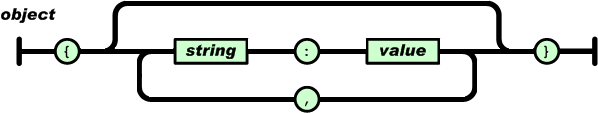
\includegraphics{img/json_obj.png}}
\end{center}
  \caption{Objeto JSON}
  \label{fig:json_obj}
\end{figure}

As definições detalhadas de cada um dos tipos e exemplos de código podem ser encontrados no site
http://www.json.org/.

\subsubsection{Web Services}

A W3C \footnote{http://www.w3c.org/} define \emph{web services} como um padrão que provê a
interoperabilidade entre duas aplicações de software, rodando sob diferentes plataformas e/ou
frameworks.
A interoperabilidade fornecida pelos \emph{web services} é disponibilizada por meio de funções
ou mesmo objetos na web, de forma que estes possam ser chamados através de um \emph{HTTP
request} e sua resposta retornada através de um \emph{HTTP response}.
Para que uma aplicação consiga se comunicar com a outra é necessário que ela conheça
e entenda o formato de entrada e saída de dados; para isso, costuma ser utilizado XML ou JSON.
Outro problema é que a aplicação deve saber qual o tipo de dados de um determinado
valor que chega a ela, e como ela implementa este valor. Este problema pode ser resolvido
de formas distintas; uma delas é a especificação trazer as informações necessárias; a outra
é o uso de um arquivo que trás esse tipo de informação, te tal forma que a aplicação
apenas leia este arquivo e faça as conversões necessárias. 


\section{Bibliotecas Utilizadas}
\label{sec:bibs}

\subsection{Reconhecimento de Texto - Tesseract-OCR}

O reconhecimento de texto em imagens digitalizadas é parte
fundamental do projeto {\it webscan}, pois somente com o uso desta 
tecnica é possível se gerar documentos com páginas indexáveis.

Após pesquisar diversas bibliotecas (pesquisa apresentada no relatório I)
a biblioteca escolhida foi a 
Tesseract-OCR\footnote{http://code.google.com/p/tesseract-ocr}, que atualmente
possui código aberto e é mantida por um grande grupo.


\subsection{Exposição de métodos - Django}
O framework Python adotado para a exposição HTTP da lib {\it webscan} foi 
Django, pois além proporcionar recursos para um desenvolvimento ágil de 
aplicações Web ele ainda facilita a organização do código fonte de aplicações
deste tipo.
 
A separação de interesses sugerida nesse framework possui uma nomenclatura 
sutilmente diferente da nomenclatura comumente adotada por vários frameworks 
de aplicações Web. 

Ao invés do conhecido MVC (Model View and Controller) utiliza-se 
MTV (Model Template and View) assim o elemento `View' do MVC chama-se 
`Template' no MTV e o `Controller' do MVC chama-se `View' no MTV, dos 
quais o {\it webscan} utiliza apenas o elemento `View'. 

Consulte a documentação oficial\footnote{http://docs.djangoproject.com/en/dev/}
para informações detalhadas sobre Django.

\subsubsection{Processamento de requisições Web}

As requisições Web são mapeadas para uma 'View' através do arquivo urls.py.
Nesse arquivo podemos configurar expressões regulares que identificam cada 
uma das urls e associam a uma determinada função de callback (View). O 
código abaixo é um trecho do arquivo urls.py do módulo server do 
{\it webscan}: 

\begin{figure}[ht]
\begin{center}
\scalebox{0.65} {
    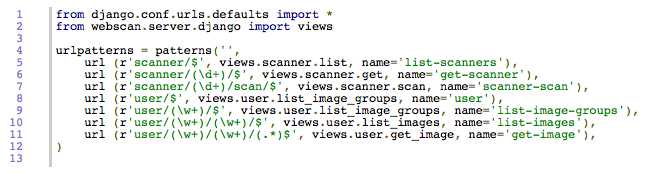
\includegraphics{imagens/urls.png}}
\end{center}
  \caption{Mapeamento de URL's - urls.py}
  \label{fig:urls}
\end{figure}

\subsection{Geração de PDF - Reportlab}

A biblioteca utilizada para geração de PDF foi a reportlab.
O código-fonte abaixo implementa a ação que gera um documento PDF apartir da 
imagem proviniente de um {\it pipeline} e seu respectivo texto OCR, se 
disponível.

\begin{figure}[ht]
\begin{center}
\scalebox{0.65} {
    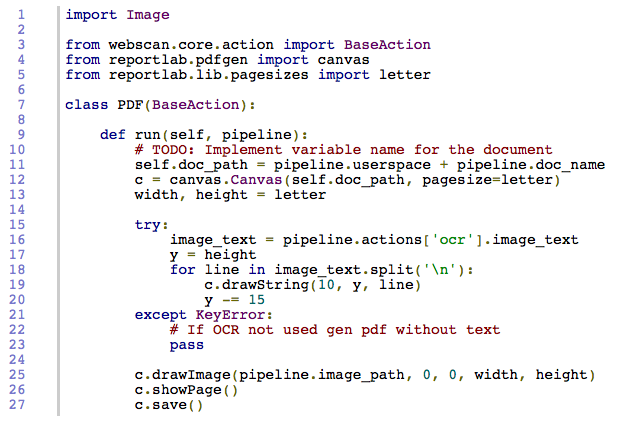
\includegraphics{imagens/pdf.png}}
\end{center}
  \caption{Action geradora de PDF's - pdf.py}
  \label{fig:urls}
\end{figure}


\subsection{Interface Web - JQuery}

O módulo UI, o qual é implementada a interface do projeto, utiliza-se apenas
de tecnologias web {\it client-side} tais como HTML, Javascript e CSS.

A utilização destas tecnologias, teoricamente, viabilizam a execução deste
artefato em qualquer plataforma que possua um navegador web compatível com elas,
porém esbarrando no problema de compatibilidade e adoção dos padrões 
internacionais W3C e ECMA.

Para que estes problemas fossem reduzidos a biblioteca 
JQuery\footnote{http://www.jquery.com} foi utilizada.
Em seu núcleo, a JQuery, implementa {\it wrappers} para os diferentes métodos
e detalhes implementados por cada navegador, ficando assim responsável por
garantir a compatibilidade do Javascript nos navegadores mais utilizados.

\section{Modularização}
\label{sec:modulos}


\subsection{Lista de diretórios e arquivos}

{\small 
\begin{verbatim}
webscan
|-- ui
|   |-- index.html
|   |-- jquery-1.2.6.js
|   `-- scanner.js
`-- daemon
    |-- setup.py
    `-- webscan
        |-- __init__.py
        |-- lib
        |   |-- __init__.py
        |   |-- conf
        |   |   |-- __init__.py
        |   |   `-- global_settings.py
        |   |-- contrib
        |   |   |-- __init__.py
        |   |   |-- action
        |   |   |   |-- __init__.py
        |   |   |   |-- ocr.py
        |   |   |   `-- pdf.py
        |   |   `-- wrapper
        |   |       |-- Sane.py
        |   |       `-- __init__.py
        |   `-- core
        |       |-- __init__.py
        |       |-- action.py
        |       |-- driver_wrapper.py
        |       |-- scanners
        |       |   |-- __init__.py
        |       |   `-- scanners.py
        |       |-- type.py
        |       `-- user.py
        `-- server
            |-- __init__.py
            `-- django
                |-- __init__.py
                |-- example
                |   |-- __init__.py
                |   |-- manage.py
                |   |-- settings.py
                |   `-- urls.py
                |-- urls.py
                |-- utils.py
                `-- views
                    |-- __init__.py
                    |-- scanner.py
                    `-- user.py
\end{verbatim}}

\subsection{Módulo Daemon}
Este módulo é responsável pela interface com drivers dos scanners, 
execução de ações, escrita de arquivos em discos além de expor todos 
os métodos relevantes como webservices.

Todos os webservices utilizados retornam JSON e estão preparados para
serem executados através de chamadas 
cross-domain\footnote{http://en.wikipedia.org/wiki/Cross\_Domain\_Solutions}.

\subsubsection{Descrição de arquivos}

Os arquivos \_\_init\_\_.py são inicializadores de pacotes padrões na linguagem 
python e por este motivo não serão detalhados neste documento. Maiores detalhes
sobre o funcionamento de pacotes em python podem ser encontrados na documentação
oficial da 
linguagem\footnote{http://docs.python.org/tutorial/modules.html\#packages}.

\begin{itemize}
\item setup.py
\begin{verbatim}
Arquivo de instalação do projeto. Neste arquivo são definidos
os metadados utilizados para a geração de pacotes e instalação
do software. Este arquivo segue o padrão setuptools.
\end{verbatim}

\item webscan/
\begin{verbatim}
Diretório que contém todo o código-fonte do módulo daemon.
Este diretório é utilizado apenas para manter separação entre
os arquivos de instalação e dos arquivos fonte.  
\end{verbatim}

\item webscan/lib/
\begin{verbatim}
Contém tudo o que for utilizado por servidores para a execução
das tarefas de escaneamento e escrita em disco.
\end{verbatim}

\item webscan/lib/conf/
\begin{verbatim}
Contém o arquivo de configuração default.
\end{verbatim}

\item webscan/lib/conf/global\_settings.py
\begin{verbatim}
Arquivo de configuração default.
\end{verbatim}

\item webscan/lib/contrib/
\begin{verbatim}
Diretório que pode vir a receber arquivos externos
acopláveis ao sistema(como plugins).
\end{verbatim}

\item webscan/lib/contrib/action/
\begin{verbatim}
Contém as ações padrões que podem ser aplicadas em imagens 
sucessivamente.
\end{verbatim}

\item webscan/lib/contrib/action/ocr.py
\begin{verbatim}
Ação que extrai conteúdo textual das imagens.
\end{verbatim}

\item webscan/lib/contrib/action/pdf.py
\begin{verbatim}
Ação responsável pela geração de PDF's a partir de imagens. 
Pode ser utilizada em conjunto com a ação ocr para gerar 
documentos indexáveis.
\end{verbatim}

\item webscan/lib/contrib/wrapper/
\begin{verbatim}
Local onde ficam todos os wrappers para drivers e 
especificações de quando eles devem ser utilizados.
\end{verbatim}

\item webscan/lib/contrib/wrapper/Sane.py
\begin{verbatim}
Wrapper para os drivers sane. Utilizado em sistemas posix.
\end{verbatim}

\item webscan/lib/contrib/wrapper/Twain.py
\begin{verbatim}
Wrapper para os drivers Twain. Utilizado nas plataformas 
Windows.
\end{verbatim}

\item webscan/lib/core/
\begin{verbatim}
Núcleo do sistema responsável pelo processamento de ações, 
imagens, além de prover classes abstratas para criação de 
ações e wrappers.
\end{verbatim}

\item webscan/lib/core/action.py
\begin{verbatim}
Instruções responsáveis pelo processamento de ações.
\end{verbatim}

\item webscan/lib/core/driver\_wrapper.py
\begin{verbatim}
Classe abstrata para a construção de um wrapper.
\end{verbatim}

\item webscan/lib/core/type.py
\begin{verbatim}
Estruturas de dados utilizadas no projeto.
\end{verbatim}

\item webscan/lib/core/user.py
\begin{verbatim}
Rotinas criadas para tratar do espaço de usuário, incluindo
grupos de imagens e escrita em disco.
\end{verbatim}

\item webscan/lib/core/scanners/
\begin{verbatim}
Implementa o singleton coleção de scanners.
\end{verbatim}

\item webscan/lib/core/scanners/scanners.py
\begin{verbatim}
Funções utilizadas pela coleção de scanners.
\end{verbatim}

\item webscan/server/
\begin{verbatim}
Espaço reservado para implementação de métodos para a 
exposição da API, via HTTP.
\end{verbatim}

\item webscan/server/django/
\begin{verbatim}
Aplicação Django criada para expor os métodos do projeto
via HTTP.
\end{verbatim}

\item webscan/server/django/urls.py
\begin{verbatim}
Arquivo de mapeamento de URL's para funções (views).
\end{verbatim}

\item webscan/server/django/utils.py
\begin{verbatim}
Funções utilizadas por mais de uma view.
\end{verbatim}

\item webscan/server/django/example/
\begin{verbatim}
Instância exemplo da aplicação Django.
\end{verbatim}

\item webscan/server/django/example/manage.py
\begin{verbatim}
Arquivo criado, automaticamente, ao se criar um projeto 
Django.
\end{verbatim}

\item webscan/server/django/example/settings.py
\begin{verbatim}
Arquivo de configuração de um projeto Django.
\end{verbatim}

\item webscan/server/django/example/urls.py
\begin{verbatim}
Arquivo base de mapeamento de urls. Default em projetos 
Django.
\end{verbatim}

\item webscan/server/django/views/
\begin{verbatim}
Métodos wrappers utilizados para chamar funções do 
webscan.lib e modificar as saídas para formatos esperados
pelo Django.
\end{verbatim}

\item webscan/server/django/views/scanner.py
\begin{verbatim}
Implementa os wrappers necessários à implementação, dos 
métodos do objeto scanner utilizando Django.
\end{verbatim}

\item webscan/server/django/views/user.py
\begin{verbatim}
Implementa os wrappers das funções relacionadas diretamente
ao usuários do sistema.
\end{verbatim}

\end{itemize} 

\subsection{Módulo UI}
O módulo UI implementa a interface web utilizada para fazer chamadas assíncronas
ao módulo daemon. 

Este módulo é composto apenas por arquivos Javascript e HTML e utiliza a biblioteca Jquery
apresentada na seção \ref{sec:bibs}.

Segue abaixo algumas capturas de tela da interface desenvolvida.

\begin{figure}[ht]
\begin{center}
\scalebox{0.5} {
    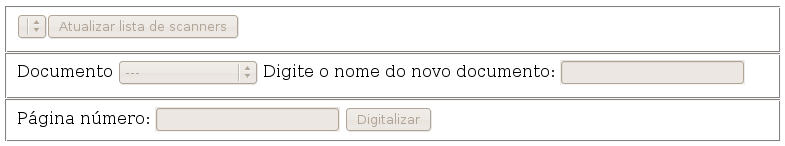
\includegraphics{imagens/lista_scanners.png}}
\end{center}
  \caption{Procura de scanners disponíveis}
  \label{fig:urls}
\end{figure}

\begin{figure}[ht]
\begin{center}
\scalebox{0.5} {
    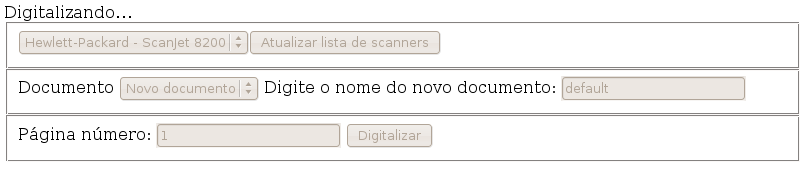
\includegraphics{imagens/digitalizando.png}}
\end{center}
  \caption{Digitalizando página em um novo documento}
  \label{fig:urls}
\end{figure}

\begin{figure}[ht]
\begin{center}
\scalebox{0.5} {
    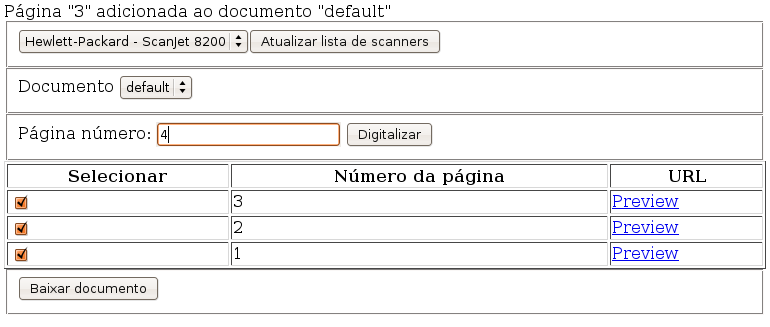
\includegraphics{imagens/digitalizado.png}}
\end{center}
  \caption{Mensagem de sucesso e lista de páginas digitalizadas}
  \label{fig:urls}
\end{figure}

\section{Considerações Finais}
\label{sec:consideracoes}

Ao aliar as informações apresentadas neste documento, documentação interna 
(de código) e documentações oficiais das bibliotecas de terceiros,
utilizadas na implementação do {\it webscan}, futuros desenvolvedores
têm as informações necessárias para dar continuidade e manutenção no projeto.

O código fonte do produto, incluindo sua respectiva documentação interna, 
pode ser encontrado no CD que acompanha este relatório e
também no repositório do projeto Interlegis: \\
http://repositorio.interlegis.gov.br/digidoc/branches/1.0/ .

Apesar da versão 1.0 do projeto ter sido entregue o projeto terá continuidade
como software livre e seu código-fonte atualizado poderá ser baixado através do
repositório do Google Code \footnote{http://webscan.googlecode.com/trunk/}
ou pelo link (svn:externals) presente no repositório interlegis: \\
http://repositorio.interlegis.gov.br/digidoc/trunk/ .

\section{Glossário}

\subsection{Atividade de Desenvolvimento:}
Atividade de desenvolvimento se refere à quantidade de escritas (ou seja, código sendo atualizado/adicionado) em um sistema de controle de versões, quando disponível.

\begin{description}
	\item[Alta:] diversas atividades no último mês.
	\item[Baixa:] algumas atividades ao longo dos últimos 3 meses.
	\item[Parado:] não houve nenhuma atividade de escrita nos últimos 6 meses.
\end{description}

\end{document}
